\documentclass[10pt,a4paper,twocolumn]{article}

\usepackage[utf8]{inputenc}
\usepackage[T1]{fontenc}
\usepackage{lmodern}
\usepackage[margin=1.55cm,columnsep=0.62cm]{geometry}
\usepackage{microtype}
\usepackage{graphicx}
\usepackage{booktabs}
\usepackage{tabularx}
\usepackage{array}
\usepackage{amsmath}
\usepackage{amssymb}
\usepackage{xcolor}
\usepackage{enumitem}
\usepackage{listings}
\usepackage[hidelinks]{hyperref}
\usepackage[font=small,labelfont=bf]{caption}

\setlength{\parindent}{0pt}
\setlength{\parskip}{0.38em}
\setlist{nosep,leftmargin=*}
\captionsetup{skip=3pt}
\renewcommand{\arraystretch}{1.08}

\lstset{
  basicstyle=\ttfamily\footnotesize,
  breaklines=true,
  frame=single,
  columns=fullflexible,
  keepspaces=true
}

\newcommand{\course}{Fundamentals of Natural Language / NLP-I}
\newcommand{\team}{Team 10}
\newcommand{\repo}{\url{https://github.com/david06redrejo-bot/FNL-Project}}
\newcommand{\kaggle}{\url{https://www.kaggle.com/competitions/uab-asho-ai-codification}}

\title{\vspace{-1.2em}\textbf{ICD-10 Category Codification from Clinical Literals using Classical NLP Baselines and Biomedical RoBERTa}}
\author{
  \team\\
  Phoebe Iglesias (1713459), David Redrejo (1790336), Pau Rossell (1750424)\\
  BSc Artificial Intelligence, Universitat Autònoma de Barcelona\\
  \course, Academic year 2025--2026\\
  Supervisors: Ernest Valveny and Lei Kang\\
  Presentation: Wednesday, June 3rd\\
  Repository: \repo \quad Competition: \kaggle
}
\date{}

\begin{document}
\maketitle

\begin{abstract}
This report describes our solution for the Kaggle competition \emph{UAB-ASHO AI Codification}. The task is to predict exactly one ICD-10 category prefix, \texttt{y\_category}, from a short clinical literal. We built the project as a sequence of decisions rather than a single model jump: first data and annotation analysis, then conservative preprocessing, classical vector-space baselines, biomedical Spanish RoBERTa fine-tuning, imbalance-aware variants, error analysis, and finally a diverse ensemble. Our best verified public Kaggle score in the repository is 0.587, obtained with \texttt{v10\_vote\_diverse\_no\_retrieval}. The private/final competition ranking is not claimed because no verified evidence is stored in the repository yet. Beyond the score, the project helped us connect course concepts---corpora, regular expressions, tokenization, TF--IDF, Transformers, pretrained language models, evaluation, and ensembles---to a realistic healthcare language problem.
\end{abstract}

\section{Introduction: Why ICD Coding Matters}

ICD coding is one of those hospital processes that is easy to underestimate until we see what depends on it. Codes support clinical documentation, statistics, diagnosis-related groups (DRGs), reimbursement, hospital management, audits, and longitudinal analysis of care. Manual coding requires expertise and attention: clinical language is abbreviated, incomplete, and often written under pressure. Errors can affect not only data quality, but also administrative decisions and financial flows.

Automated ICD coding is therefore attractive, but risky. A model can help by ranking or suggesting likely categories, yet it should not replace professional coders. Our project focuses on a narrower competition task: given a clinical literal, predict the first character of the ICD code. This is much simpler than full ICD coding from complete electronic medical records. After this first observation, however, the task did not become trivial: short literals often lack context and may contain abbreviations, punctuation, accents, digits, and domain-specific shorthand.

\section{Project Context and Competition}

The project was developed for \course{} at Universitat Autònoma de Barcelona during academic year 2025--2026. The team is \team: Phoebe Iglesias, David Redrejo, and Pau Rossell. The supervisors/professors are Ernest Valveny and Lei Kang.

The competition was \emph{UAB-ASHO AI Codification} on Kaggle~\cite{kaggleuabasho}. The expected output is a single label \texttt{y\_category} per leaderboard row. Kaggle public leaderboard feedback was useful for checking submissions, but we kept internal validation results separate from public scores to avoid telling a misleading story. After an initial baseline and short presentation, we had a follow-up with Lei Kang, who told us the direction was good. At that stage, after baseline tests, the team was around second in the competition. We include this as project context; a formal final ranking claim should only be made after adding verified evidence such as a screenshot or official table.

\section{Data and Annotation Analysis}

Our first technical phase was deliberately \emph{Analyzing the data and the annotations}. This follows the Data Engineering mindset: before modeling, inspect the data-generating process, schemas, missingness, duplicates, distributions, and possible leakage. Table~\ref{tab:data} summarizes the actual files found.

\begin{table}[h]
\centering
\caption{Dataset files found in \texttt{data/raw}.}
\label{tab:data}
\begin{tabularx}{\columnwidth}{lrrX}
\toprule
File & Rows & Cols & Role \\
\midrule
\texttt{codification\_data.csv} & 13,700 & 2 & Training literals with \texttt{Code}. \\
\texttt{leaderboard\_data.csv} & 6,667 & 2 & Kaggle leaderboard literals. \\
\texttt{icd\_d\_p\_pairs.csv} & 179,742 & 3 & ICD catalogue pairs/descriptions. \\
\bottomrule
\end{tabularx}
\end{table}

The annotation contract is:
\begin{equation}
y_i = \operatorname{firstchar}(\operatorname{str}(\texttt{Code}_i)).
\end{equation}
In code, this is:
\begin{lstlisting}[language=Python]
df["y_category"] = df["Code"].astype(str).str[0]
\end{lstlisting}

The training set contains all 36 expected categories. The leaderboard file does not contain \texttt{y\_category}, which is normal for an unlabeled Kaggle test file even though the initial statement mentioned it.

The full EDA found 4,059 unique ICD codes in training and 179,742 ICD codes in the catalogue. It also found 1,668 duplicate literal groups with multiple full ICD codes, and 1,486 duplicate literal groups with multiple \texttt{y\_category} labels. Examples such as \emph{obesidad parto}, \emph{Fumadora part}, and \emph{Hipotiroidismo parto} appeared with several different codes and categories. This changed how we approached modeling: identical or nearly identical literals could not be treated as automatically solved string matches.

Figure~\ref{fig:catdist} shows the class distribution. The largest categories are much more frequent than the tail, so a model can obtain non-trivial accuracy by learning imbalance. Figure~\ref{fig:longtail} makes the long-tail shape clearer.

Table~\ref{tab:eda} records the main EDA numbers used later in the modeling decisions.

\begin{table}[h]
\centering
\caption{Key EDA values used in the report.}
\label{tab:eda}
\begin{tabularx}{\columnwidth}{Xr}
\toprule
Observation & Value \\
\midrule
Training rows & 13,700 \\
Leaderboard rows & 6,667 \\
Unique training ICD codes & 4,059 \\
Unique \texttt{y\_category} labels & 36 \\
Duplicate literal groups & 1,668 \\
Same literal, multiple categories & 1,486 \\
Leaderboard normalized literals seen in train & 51.8\% \\
Mean train literal length & 16.95 chars \\
Mean leaderboard literal length & 17.15 chars \\
\bottomrule
\end{tabularx}
\end{table}

\begin{figure}[h]
\centering
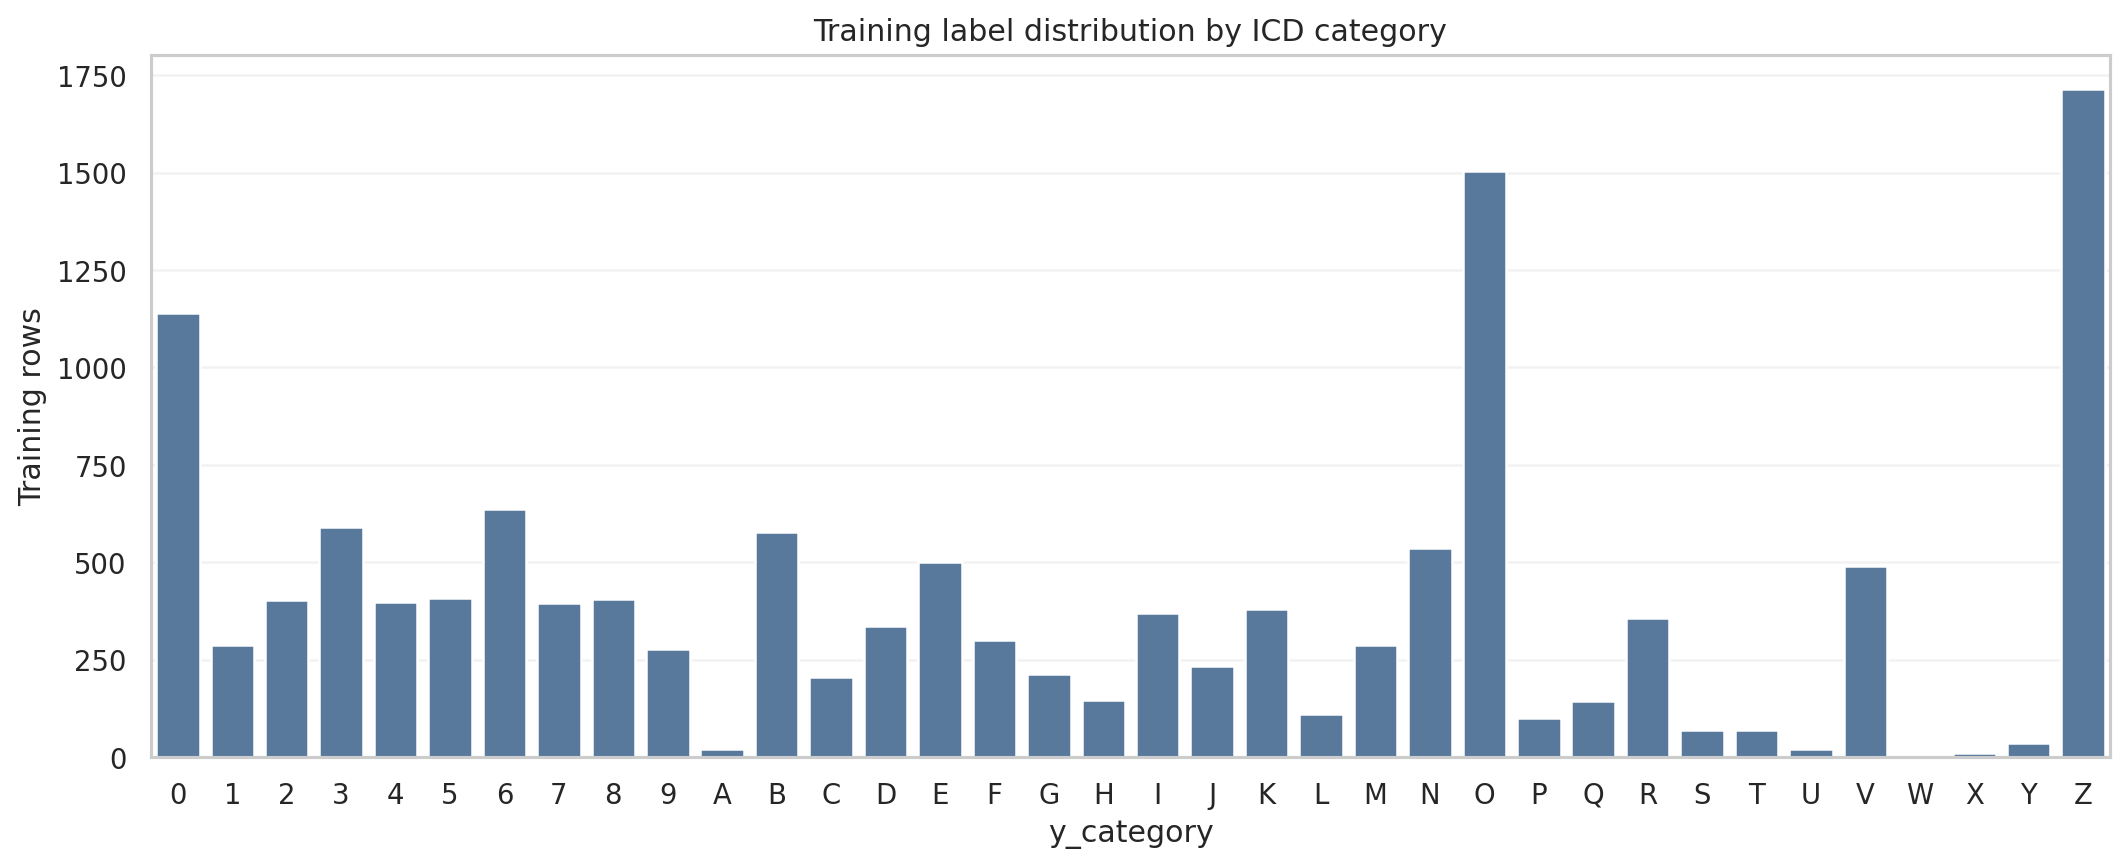
\includegraphics[width=\columnwidth]{figures/fig_01_category_distribution.png}
\caption{Training category distribution. The most frequent class is \texttt{Z}, followed by \texttt{O} and \texttt{0}.}
\label{fig:catdist}
\end{figure}

\begin{figure}[h]
\centering
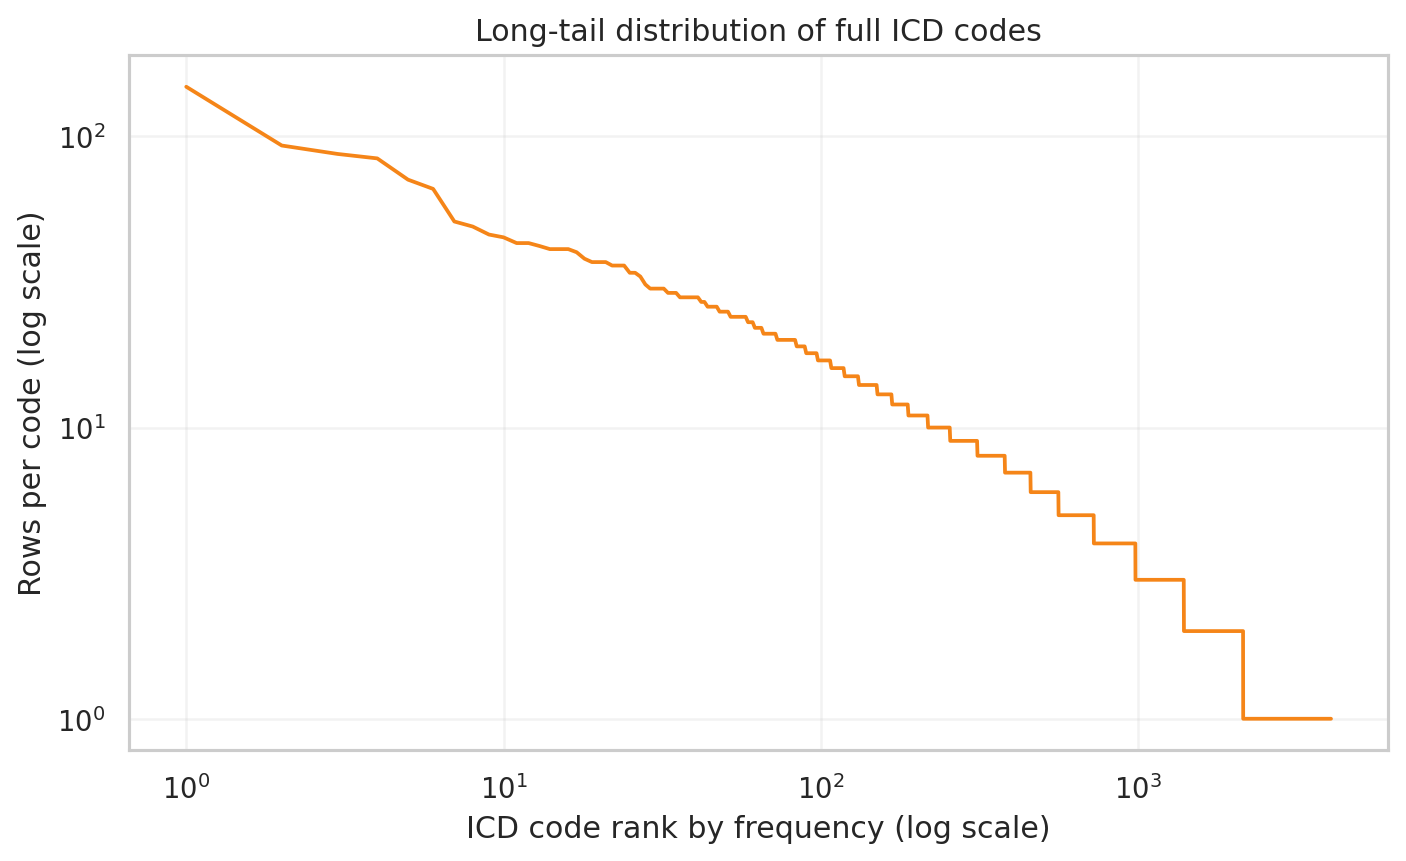
\includegraphics[width=\columnwidth]{figures/fig_02_long_tail_distribution.png}
\caption{Long-tail distribution. Rare categories motivated macro-F1 reporting and imbalance-aware experiments.}
\label{fig:longtail}
\end{figure}

\section{Understanding the Main Challenges}

The second phase was \emph{Understanding the main challenges of the task}. After the first EDA pass, the data suggested five central difficulties.

\textbf{Class imbalance.} The majority baseline already reaches 0.125 accuracy by always predicting the most frequent category. Accuracy is therefore necessary but not sufficient; macro-F1 is important to see rare-class behavior.

\textbf{Clinical ambiguity.} A short literal may refer to different clinical contexts. Unlike long EMR-based ICD coding, this task rarely gives surrounding evidence.

\textbf{Abbreviations and symbols.} Literals include uppercase shorthand, slashes, hyphens, parentheses, digits, measurements, and accents. Removing them too aggressively could destroy signal.

\textbf{Broad target.} Predicting only the first ICD character is easier than full ICD coding, but it can hide clinically different codes inside the same broad prefix.

\textbf{Train--test shift.} We can compare literal lengths and surface patterns between train and leaderboard, but we do not observe leaderboard labels. Figure~\ref{fig:lengthshift} shows that the token/length scale is similar, which reduces but does not remove distribution-shift concerns.

Figure~\ref{fig:patterns} shows that the train and leaderboard sets share similar surface patterns. In training, 27.98\% of literals contain accents, 11.83\% are all-uppercase, 9.77\% contain punctuation, and 7.98\% contain digits. The leaderboard values are close: 29.59\% accents, 11.31\% all-uppercase, 8.95\% punctuation, and 7.59\% digits. This supported the decision to preserve these signals instead of aggressively normalizing them away.

\begin{figure}[h]
\centering
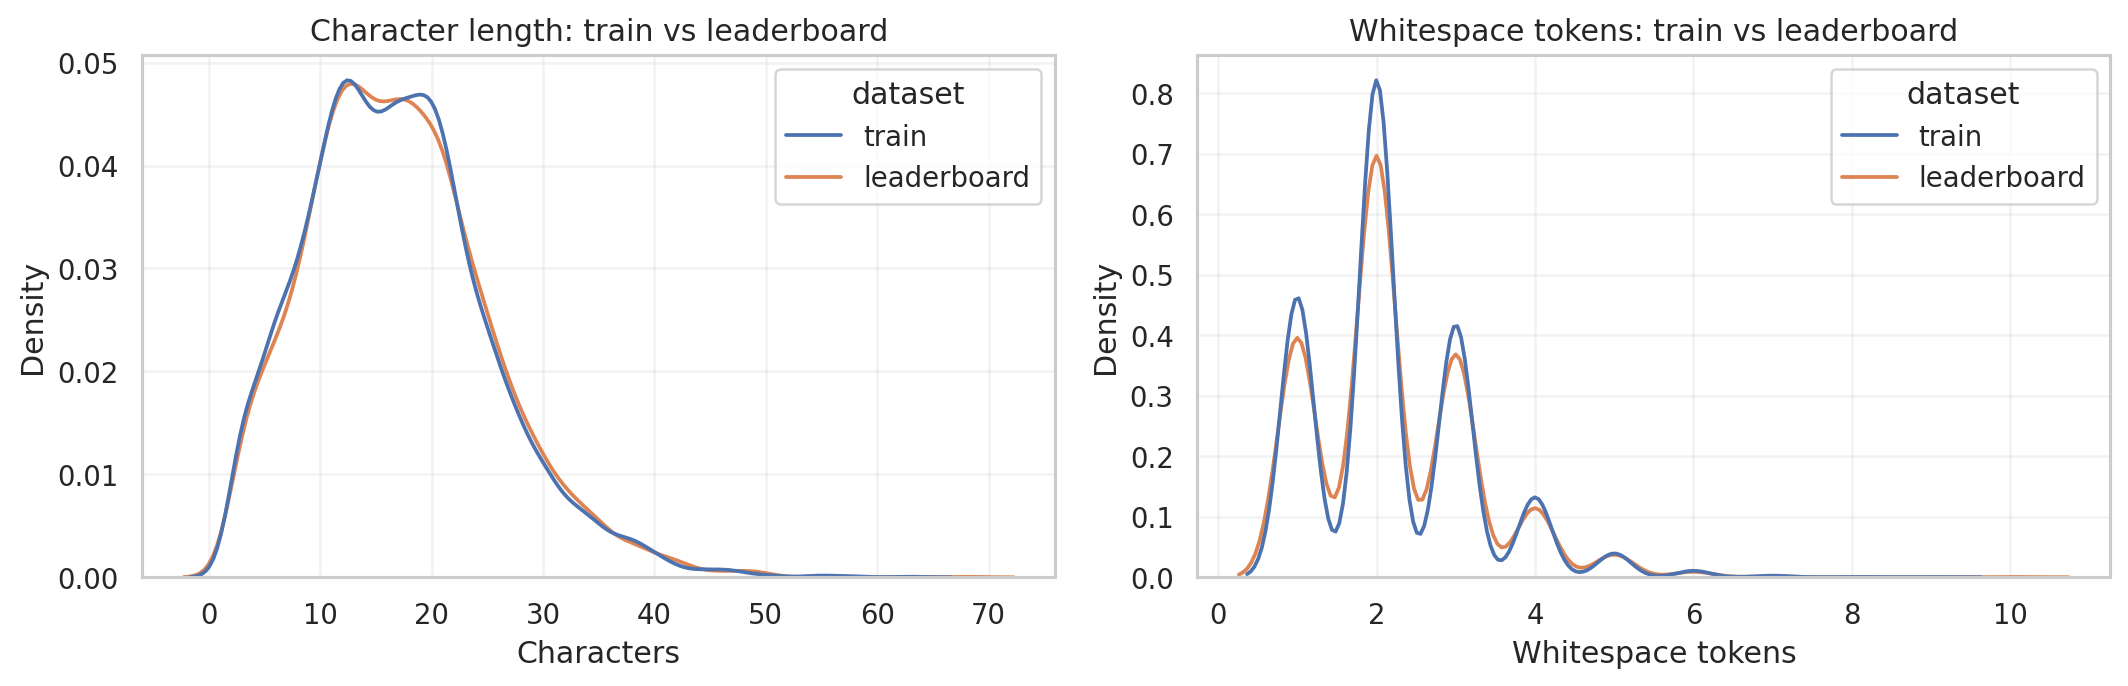
\includegraphics[width=\columnwidth]{figures/fig_05_train_vs_leaderboard_lengths.png}
\caption{Train versus leaderboard literal lengths. Both splits contain short literals, but labels are unavailable for leaderboard rows.}
\label{fig:lengthshift}
\end{figure}

\begin{figure}[h]
\centering
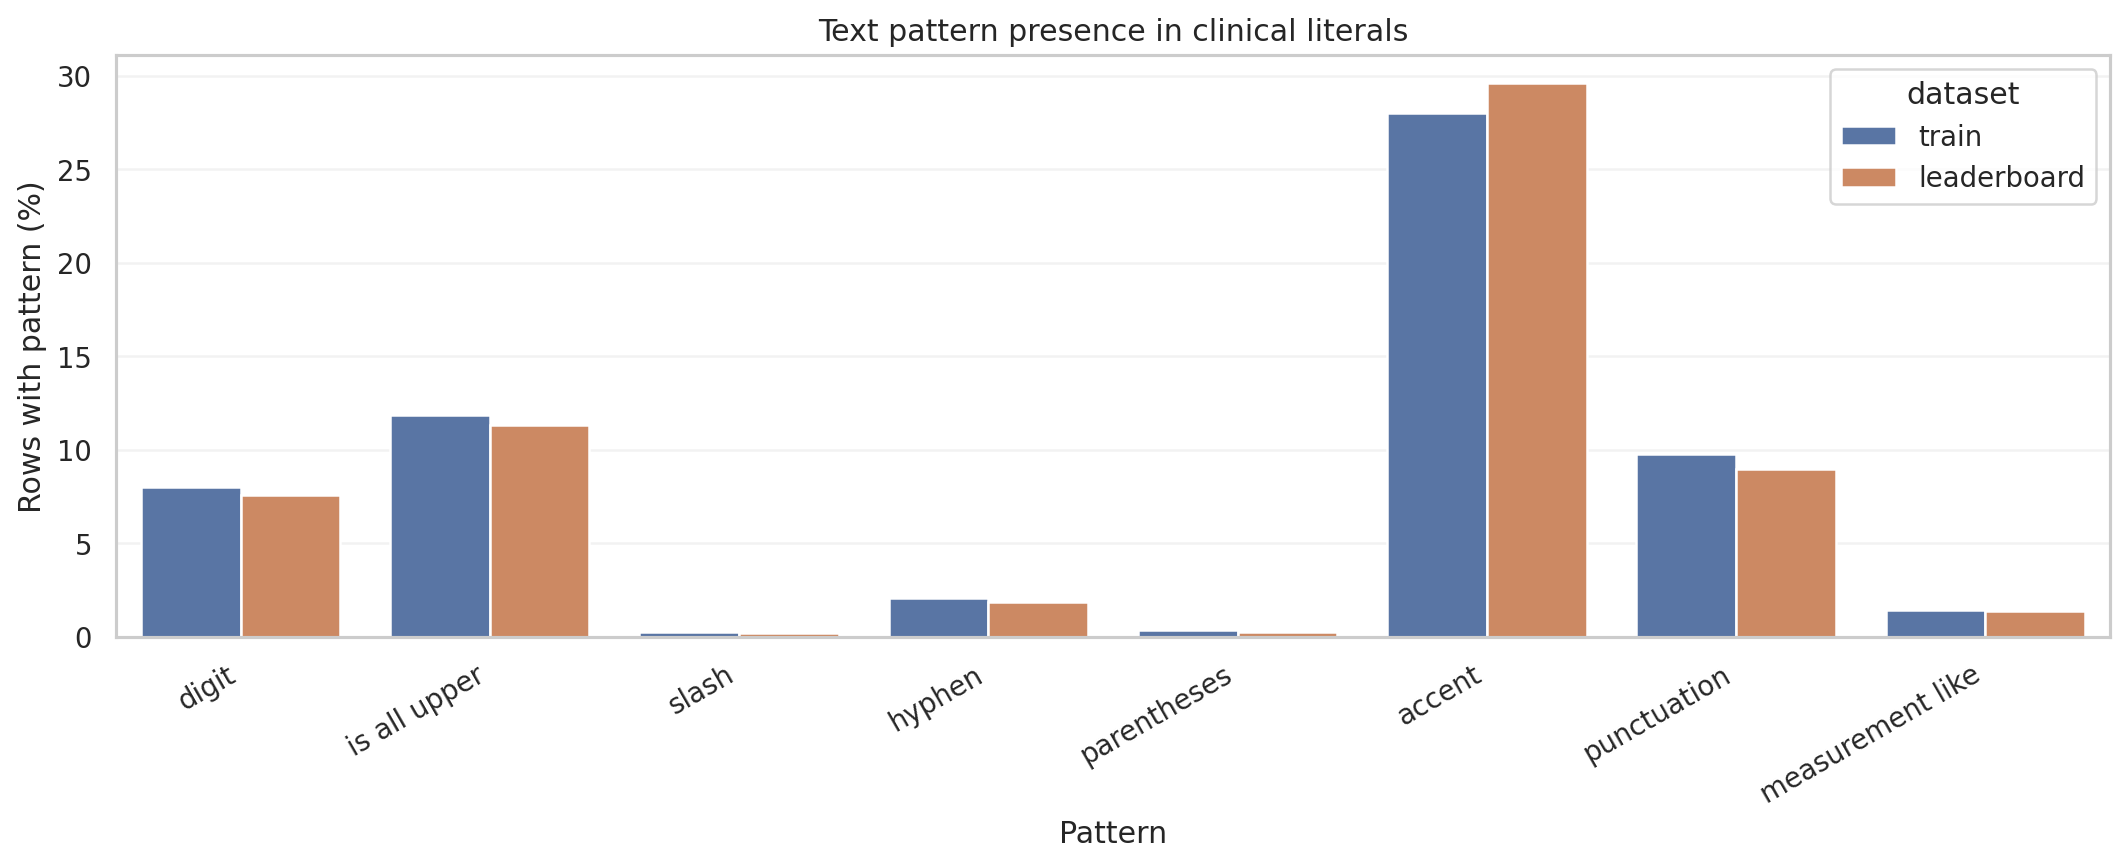
\includegraphics[width=\columnwidth]{figures/fig_06_text_pattern_presence.png}
\caption{Presence of digits, uppercase literals, accents, punctuation, and other clinical-text patterns in train and leaderboard data.}
\label{fig:patterns}
\end{figure}

\section{Course and Literature Grounding}

Yan et al.~\cite{yan2022survey} describe the evolution of automated ICD coding from rule-based systems to traditional machine learning, neural models, knowledge-based methods, and pretrained language models. They also emphasize challenges that appeared in our own project: large label spaces, unbalanced labels, long clinical documents, and interpretability. Our assignment differs because the target is a single first-character category and the input is a literal rather than a full discharge summary, but the same core tensions remain: medical terminology, imbalance, ambiguity, and trust.

We also used Spanish clinical-coding context from CodiEsp~\cite{miranda2020codiesp}. This helped us place the assignment in a broader line of non-English clinical NLP work: even though our Kaggle task is smaller than full ICD coding, it still sits inside the same practical problem of turning clinical language into standardized codes.

The project connected directly to several course topics. The EDA phase relates to corpora and linguistic datasets. Preprocessing used Basic Text Processing ideas: regular expressions, whitespace normalization, tokenization, and the danger of losing linguistic information. TF--IDF baselines connect to vector-space models and feature engineering from Fundamentals of Machine Learning. RoBERTa connects to Transformers, self-attention, pretrained language models, and fine-tuning from NLP and Neural Networks and Deep Learning~\cite{vaswani2017attention,devlin2019bert,liu2019roberta}. The final ensemble connects to the Machine Learning idea that different models may make partially uncorrelated errors.

Figure~\ref{fig:survey} summarizes how the survey's method evolution influenced our project decisions.

\begin{figure}[h]
\centering
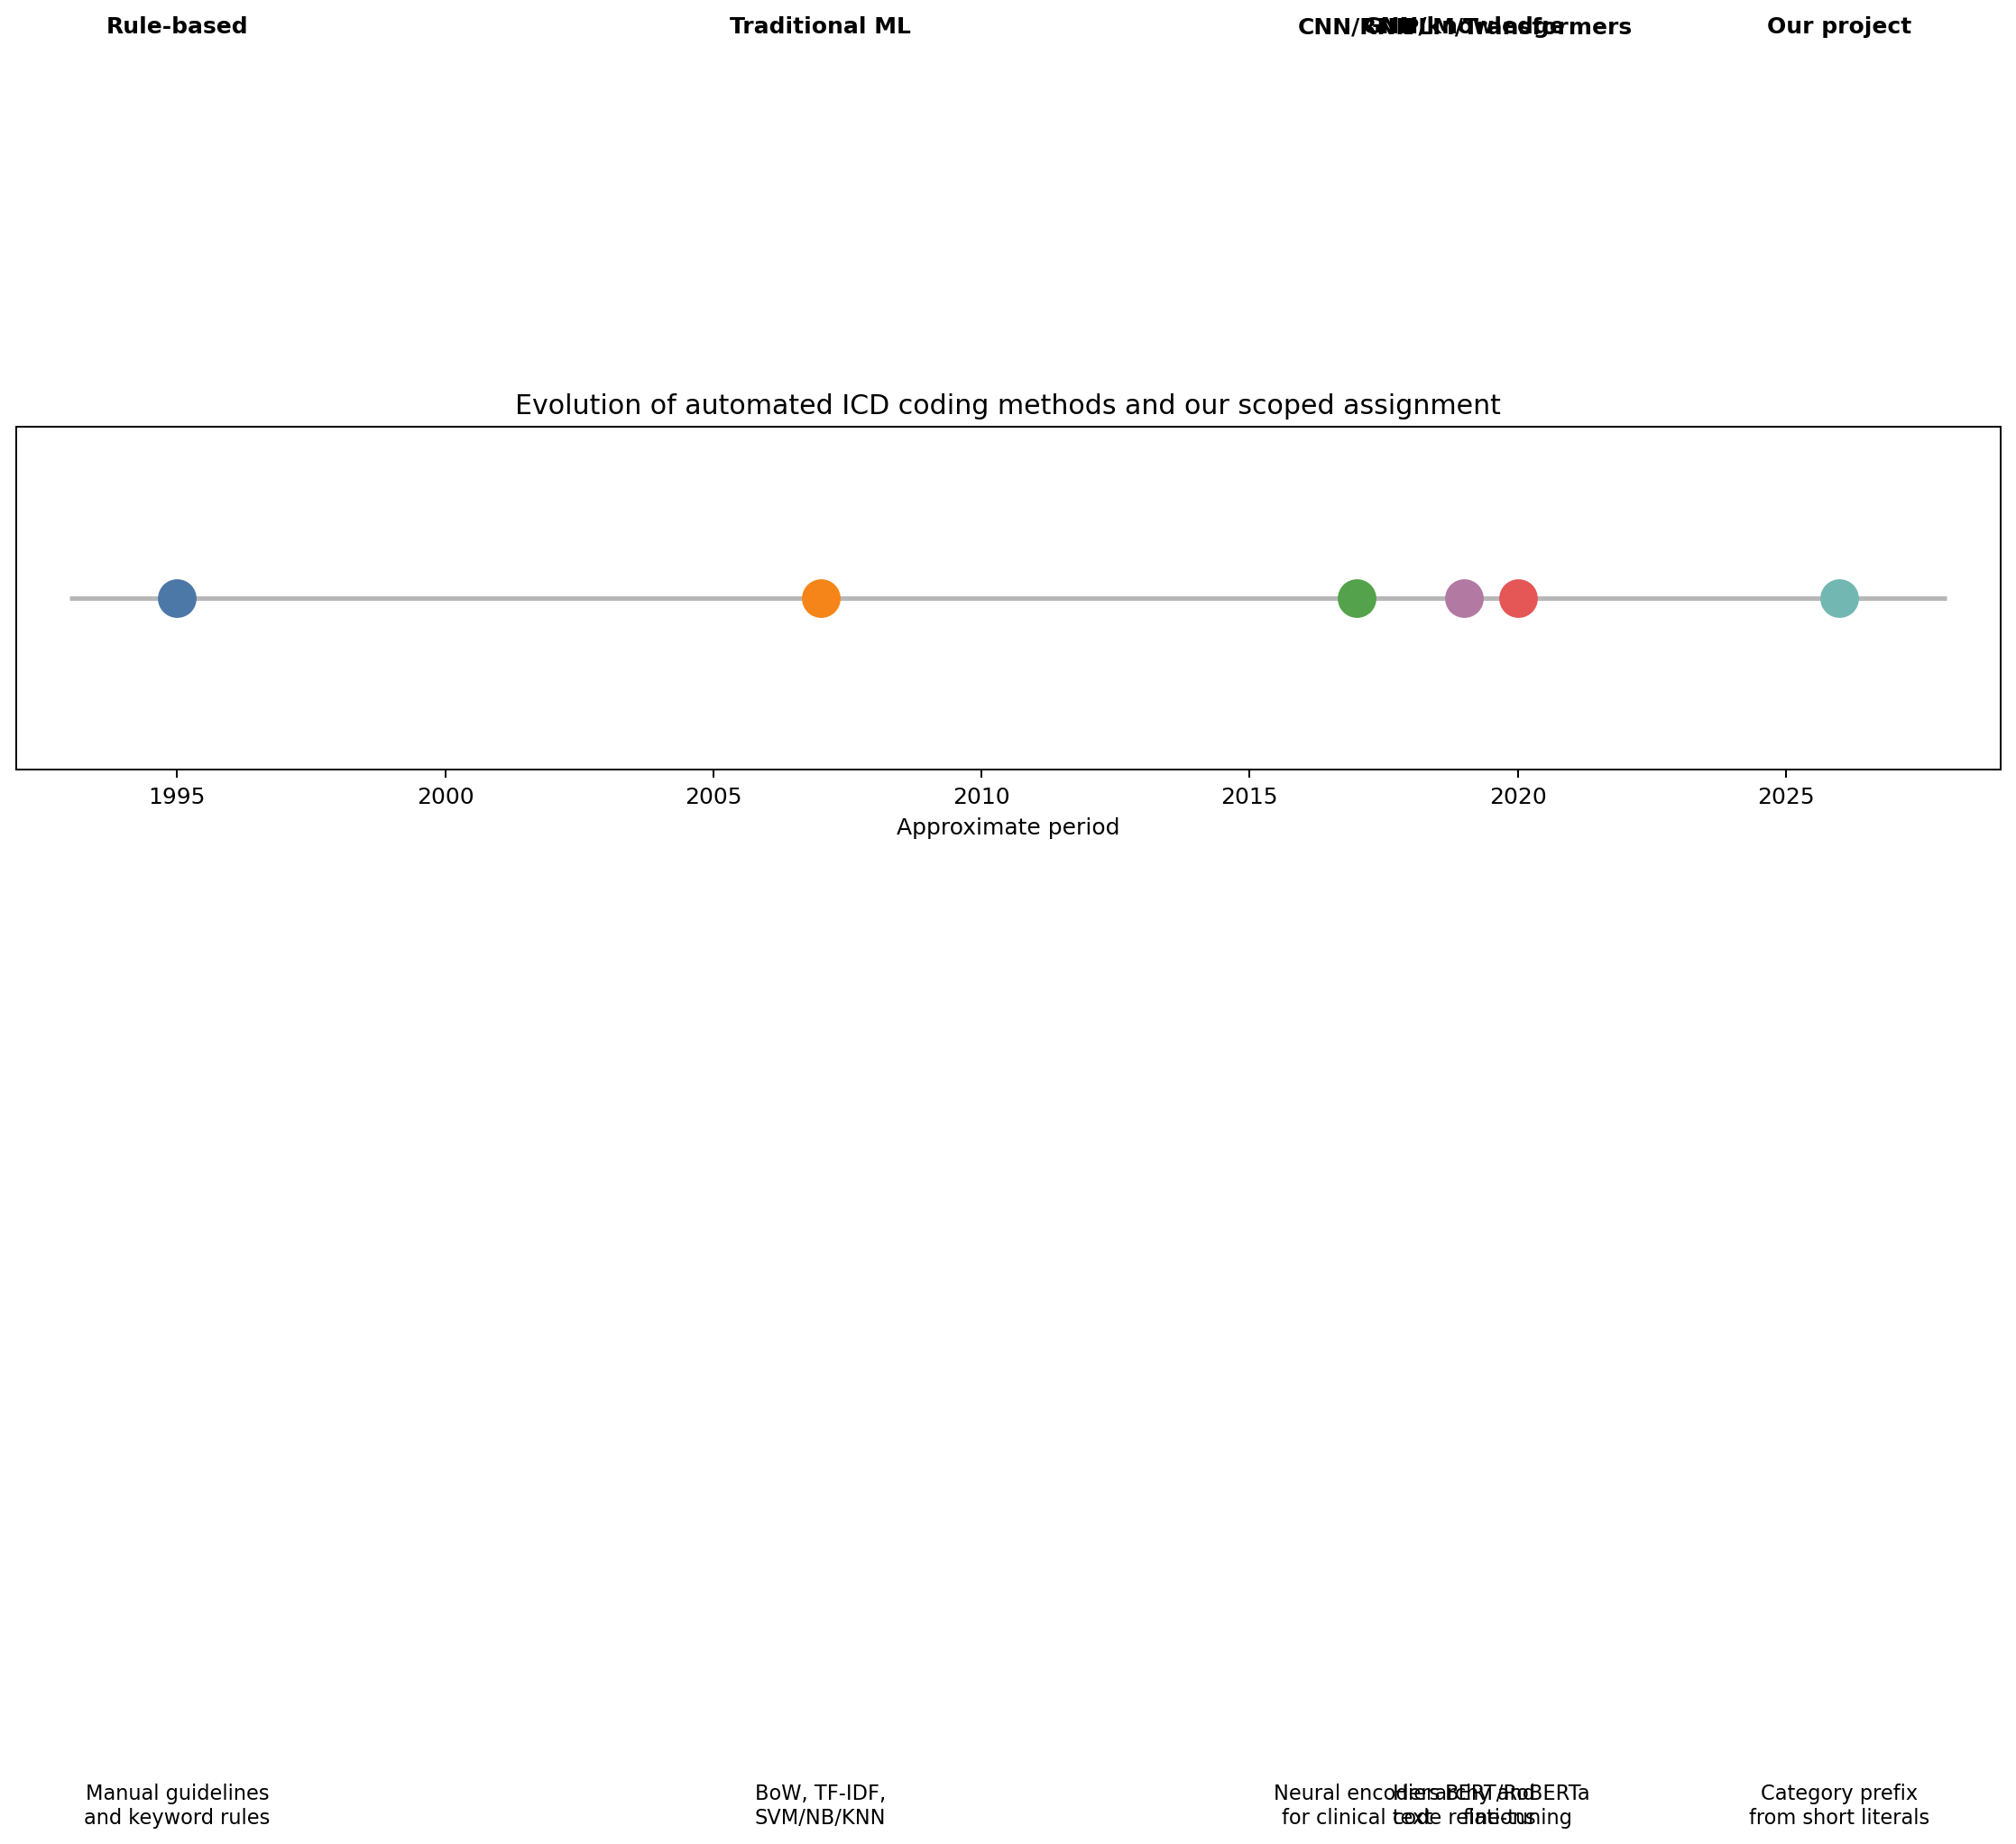
\includegraphics[width=\columnwidth]{figures/fig_09_method_evolution_timeline.png}
\caption{Method evolution from the ICD coding survey and how it guided our feasible project choices.}
\label{fig:survey}
\end{figure}

\section{Preprocessing and Annotation Design}

The final preprocessing pipeline is intentionally light:
\begin{lstlisting}[language=Python]
text = str(text)
text = text.strip()
text = re.sub(r"\s+", " ", text)
\end{lstlisting}

We did not lowercase, remove accents, or remove punctuation for the final RoBERTa pipeline. The reason is linguistic and practical: the backbone tokenizer was pretrained on Spanish biomedical and clinical text, and the EDA showed that case, accents, punctuation, digits, and abbreviations may encode medical meaning. This is why we moved from EDA to preprocessing cautiously. More aggressive normalization was treated as an ablation for classical models, not as the default.

Subword tokenization also influenced design. With \texttt{PlanTL-GOB-ES/roberta-base-biomedical-clinical-es}, the median token length was 5 tokens in both train and leaderboard, the 99th percentile was 12, and the maximum was 24 for training. We selected a default \texttt{max\_length} of 32, shown in Figure~\ref{fig:toklen}. This is a small but important example of not treating Transformer input length as arbitrary.

\begin{figure}[h]
\centering
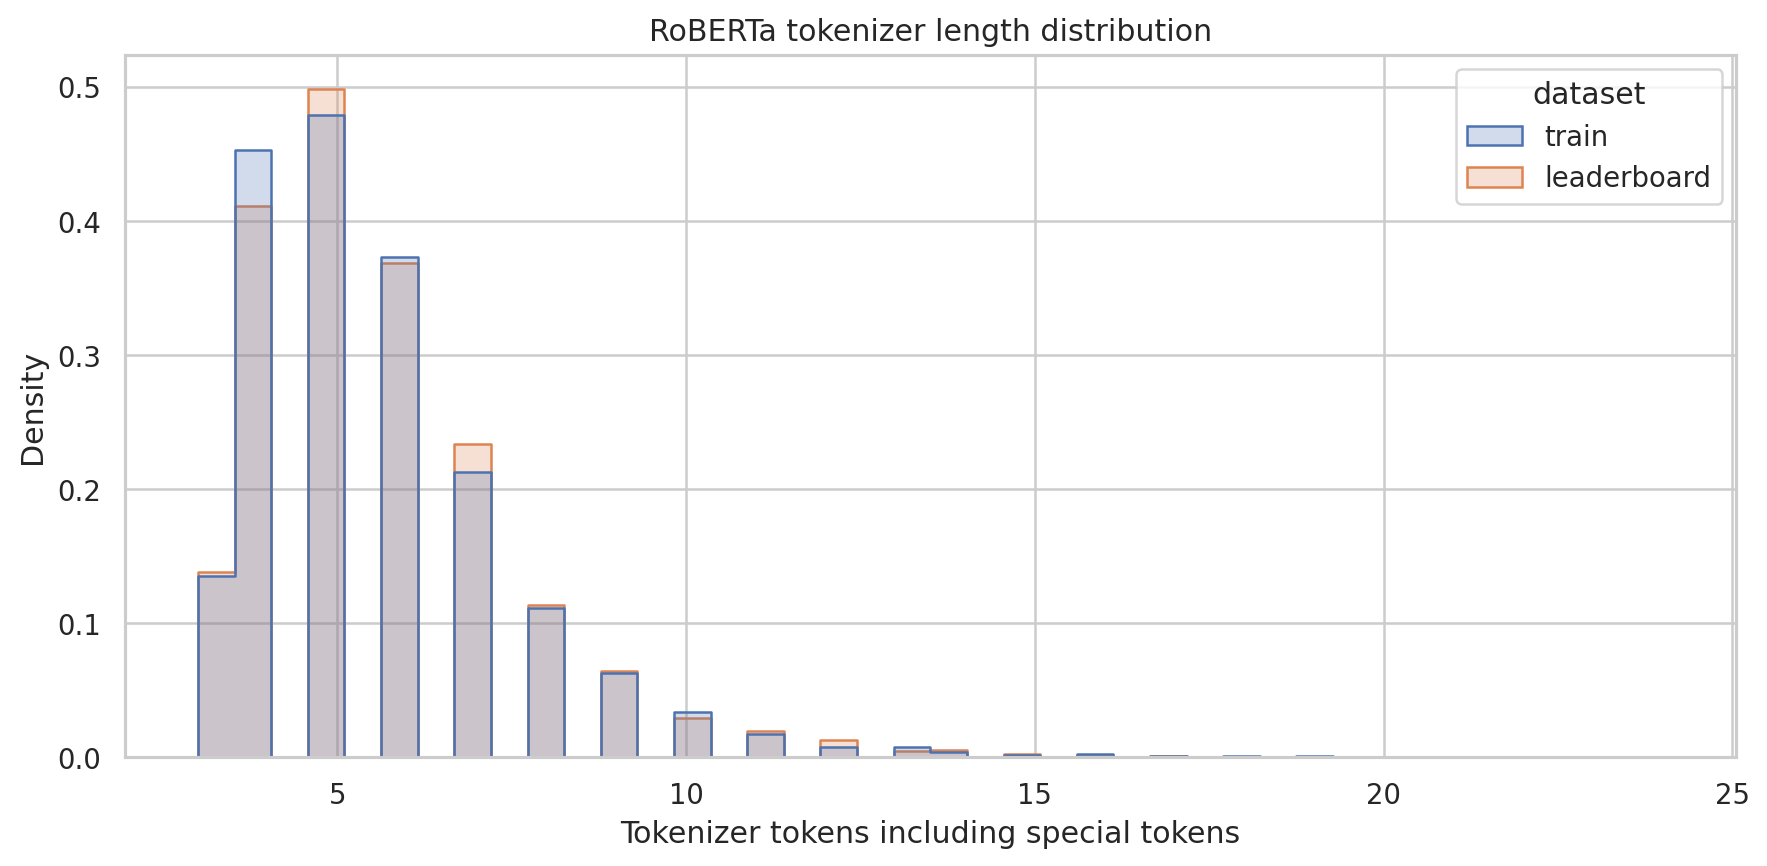
\includegraphics[width=\columnwidth]{figures/fig_07_token_length_distribution.png}
\caption{Subword token length distribution for the biomedical Spanish RoBERTa tokenizer.}
\label{fig:toklen}
\end{figure}

\section{Methodology}

We implemented each model as a runnable versioned script that loads data, creates an 80/20 stratified split, evaluates validation predictions, writes metrics, writes detailed predictions, and generates a Kaggle submission.

\textbf{Majority baseline.} \texttt{v00} predicts the most frequent training-split class for every example. It is intentionally weak but essential: it tells us how much imbalance alone explains.

\textbf{Character TF--IDF.} \texttt{v01} uses \texttt{TfidfVectorizer(analyzer="char\_wb")} with logistic regression. The EDA suggested this baseline because many useful clues live inside short words, abbreviations, fragments, and punctuation-heavy clinical literals.

\textbf{Word TF--IDF.} \texttt{v02} uses word n-grams with linear SVM/logistic alternatives. This tests whether whole-word lexical signal is enough.

\textbf{Similarity retrieval.} \texttt{v03} treats the task as nearest-neighbor retrieval over training literals using TF--IDF cosine similarity. It is intuitive and related to information-retrieval views of coding, but limited when similar strings have different labels.

\textbf{RoBERTa CLS.} \texttt{v04} fine-tunes a Spanish biomedical-clinical RoBERTa backbone. We moved to RoBERTa after the classical baselines showed that text signal existed, but sparse surface features could not fully resolve ambiguity. For CLS pooling:
\begin{equation}
\mathbf{h} = \mathbf{H}_{[:,0,:]},
\end{equation}
where the first token representation is passed through dropout and a linear classifier.

\textbf{RoBERTa mean pooling.} \texttt{v05} averages non-padding hidden states:
\begin{equation}
\mathbf{h}
= \frac{\sum_{t=1}^{T} m_t \mathbf{H}_t}{\max(1,\sum_{t=1}^{T} m_t)}.
\end{equation}
Mean pooling may help short literals because every token can contribute directly to the representation.

\textbf{Improvements.} The RoBERTa baselines improved accuracy, but rare classes and ambiguous literals remained fragile. This is why \texttt{v06} tested class-weighted cross entropy and focal loss, \texttt{v07} tuned learning rate, warmup, dropout, weight decay, batch size, gradient clipping, and AMP, and \texttt{v08} tested safe data strategies, especially duplicate handling and sampling. We avoided unsafe augmentation such as random medical-word deletion or unverified synonym replacement.

\textbf{Ensemble.} \texttt{v09} combined complementary saved models. \texttt{v10} broadened the search toward diverse Machine Learning combinations. The final public candidate, \texttt{v10\_vote\_diverse\_no\_retrieval}, is a majority vote over RoBERTa safe-dedupe mean, RoBERTa CLS, character TF--IDF logistic regression, and word TF--IDF SVM. Figure~\ref{fig:arch} shows the final architecture.

\begin{figure*}[t]
\centering
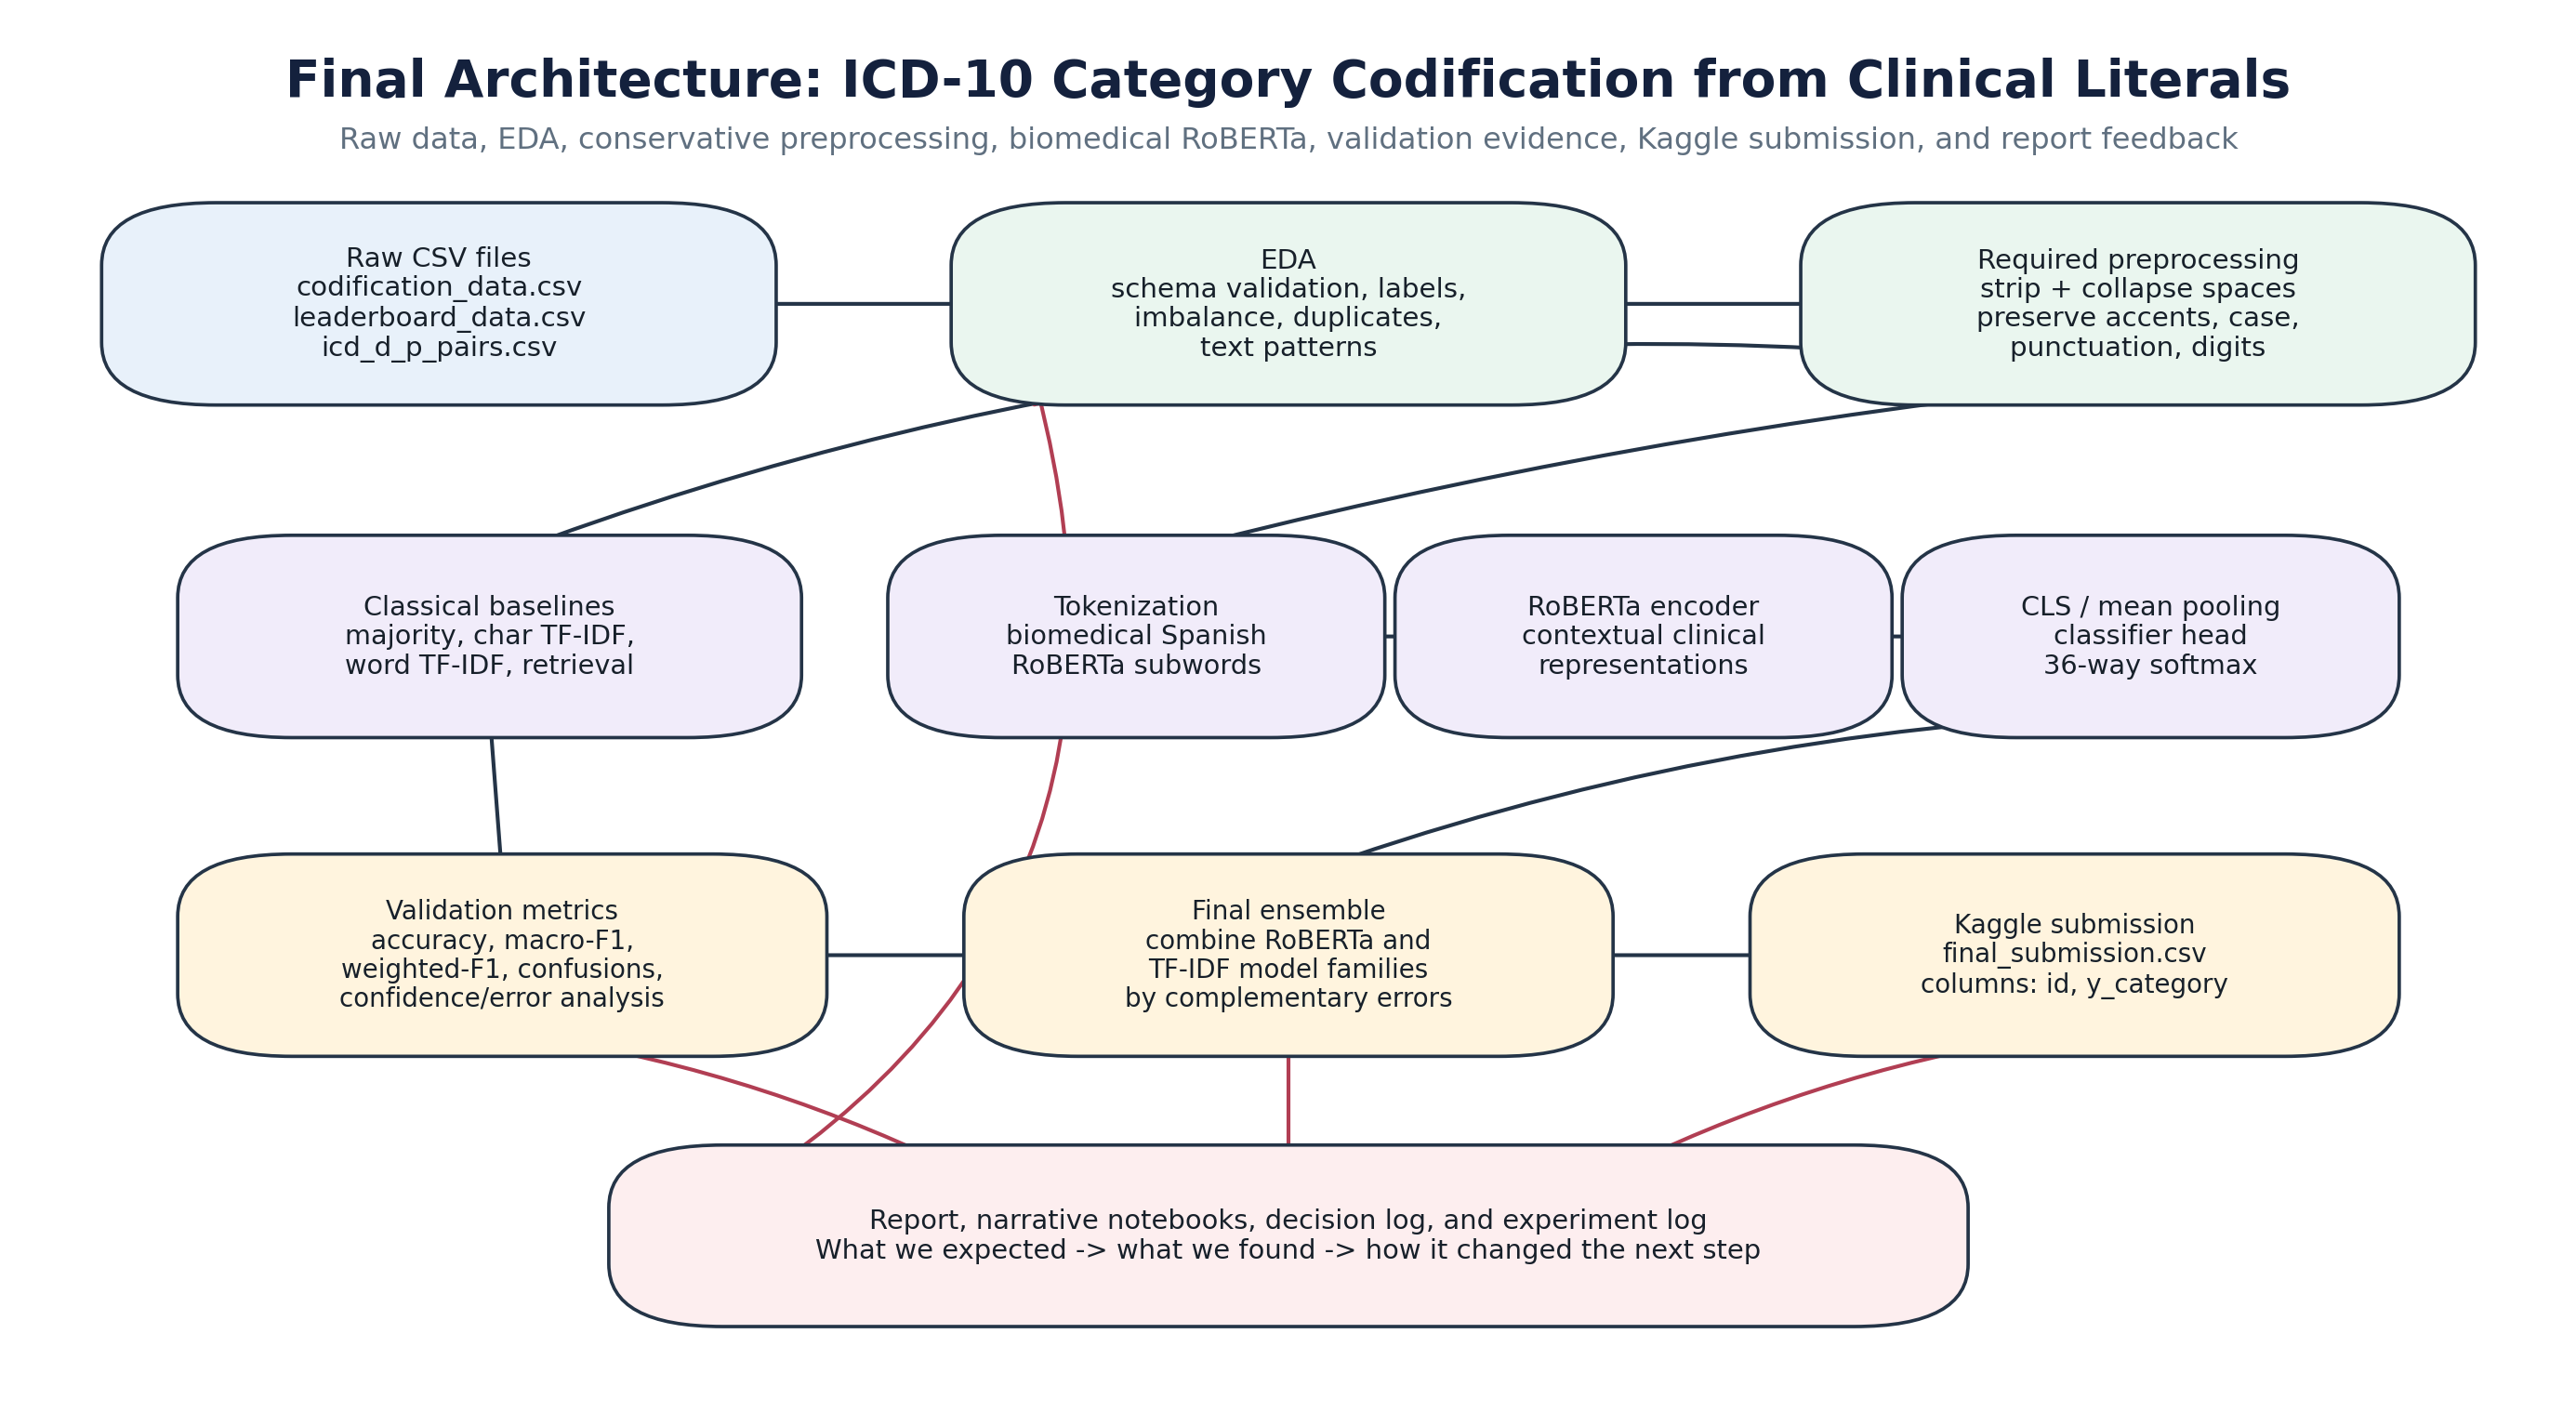
\includegraphics[width=0.92\textwidth]{figures/final_architecture_diagram.png}
\caption{Final project architecture: data, light preprocessing, tokenizer, RoBERTa backbone, pooling/classification, prediction, and the final diverse ensemble used for submission.}
\label{fig:arch}
\end{figure*}

\section{Training and Experimental Setup}

All experiments used a stratified 80/20 train/validation split by \texttt{label\_id}. Seeds were configurable and fixed in Python, NumPy, and PyTorch where applicable. Classical models were trained with scikit-learn~\cite{pedregosa2011scikit}. RoBERTa models used the Hugging Face Transformers ecosystem~\cite{wolf2020transformers} and the Spanish biomedical-clinical checkpoint from PlanTL-GOB-ES~\cite{carrino2022pretrained,plantlroberta}.

Before filling the final report, we inspected \texttt{outputs/metrics}, \texttt{outputs/logs}, \texttt{EXPERIMENT\_LOG.md}, \texttt{REPORT\_NOTES.md}, \texttt{DECISIONS.md}, and \texttt{submissions}. Files containing \texttt{debug}, \texttt{dry\_run}, or \texttt{smoke} were treated as infrastructure checks only and are not reported as final metrics. The results in Table~\ref{tab:results} come from full runs or from the consolidated final evaluation tables.

For neural models, the main setup was cross entropy loss:
\begin{equation}
\mathcal{L}
= - \frac{1}{N}\sum_{i=1}^{N}
\log \frac{\exp z_{i,y_i}}{\sum_{c=1}^{C}\exp z_{i,c}},
\end{equation}
with AdamW, learning rate \(2\cdot 10^{-5}\), weight decay \(0.01\), dropout \(0.1\), early stopping by validation accuracy, and GPU acceleration when available in the course VM environment. No credentials are stored in the repository.

We report accuracy and F1. Accuracy is:
\begin{equation}
\mathrm{Acc}=\frac{1}{N}\sum_{i=1}^{N}\mathbb{1}[\hat{y}_i=y_i].
\end{equation}
For each class \(c\):
\begin{equation}
F1_c = \frac{2P_cR_c}{P_c+R_c}.
\end{equation}
Macro-F1 averages classes equally; weighted-F1 weights by class frequency. This distinction matters because the label distribution is imbalanced.

\section{Results}

Table~\ref{tab:results} contains the main validation and public leaderboard results. The best public score verified in repository files is 0.587 for \texttt{v10\_vote\_diverse\_no\_retrieval}. The private/final ranking is not claimed.

\begin{table*}[t]
\centering
\caption{Main model comparison. Public scores are reported only when a verified Kaggle submission exists in \texttt{reports/tables/kaggle\_submission\_scores.csv}.}
\label{tab:results}
\begin{tabular}{llrrrr}
\toprule
Version & Model & Accuracy & Macro-F1 & Weighted-F1 & Public \\
\midrule
v00 & Majority baseline & 0.125182 & 0.006181 & 0.027854 & -- \\
v01 & Char TF--IDF + logreg & 0.522628 & 0.402554 & 0.494943 & 0.550 \\
v02 & Word TF--IDF + SVM & 0.520073 & 0.474196 & 0.514018 & 0.536 \\
v03 & Similarity retrieval & 0.497445 & 0.462789 & 0.496120 & -- \\
v04 & RoBERTa CLS & 0.569343 & 0.494329 & 0.554347 & 0.573 \\
v05 & RoBERTa mean & 0.564599 & 0.496567 & 0.549541 & 0.556 \\
v06 & Imbalance-aware RoBERTa & 0.557299 & 0.480394 & 0.539776 & 0.555 \\
v07 & Tuned RoBERTa mean & 0.564599 & 0.494151 & 0.549054 & 0.572 \\
v08 & Safe data strategy & 0.568613 & 0.481648 & 0.549150 & 0.583 \\
v09 & Validation ensemble & 0.576642 & \textbf{0.506277} & \textbf{0.561544} & 0.573 \\
v10 & Diverse ensemble & \textbf{0.579562} & 0.496677 & 0.561294 & \textbf{0.587} \\
\bottomrule
\end{tabular}
\end{table*}

Figure~\ref{fig:modelcomparison} visualizes the same trend. The jump from majority baseline to TF--IDF was large, which confirmed that the literals contain real lexical signal. RoBERTa improved further by adding contextual biomedical representations, and ensembles gave the best final candidates by combining both kinds of evidence.

\begin{figure}[h]
\centering
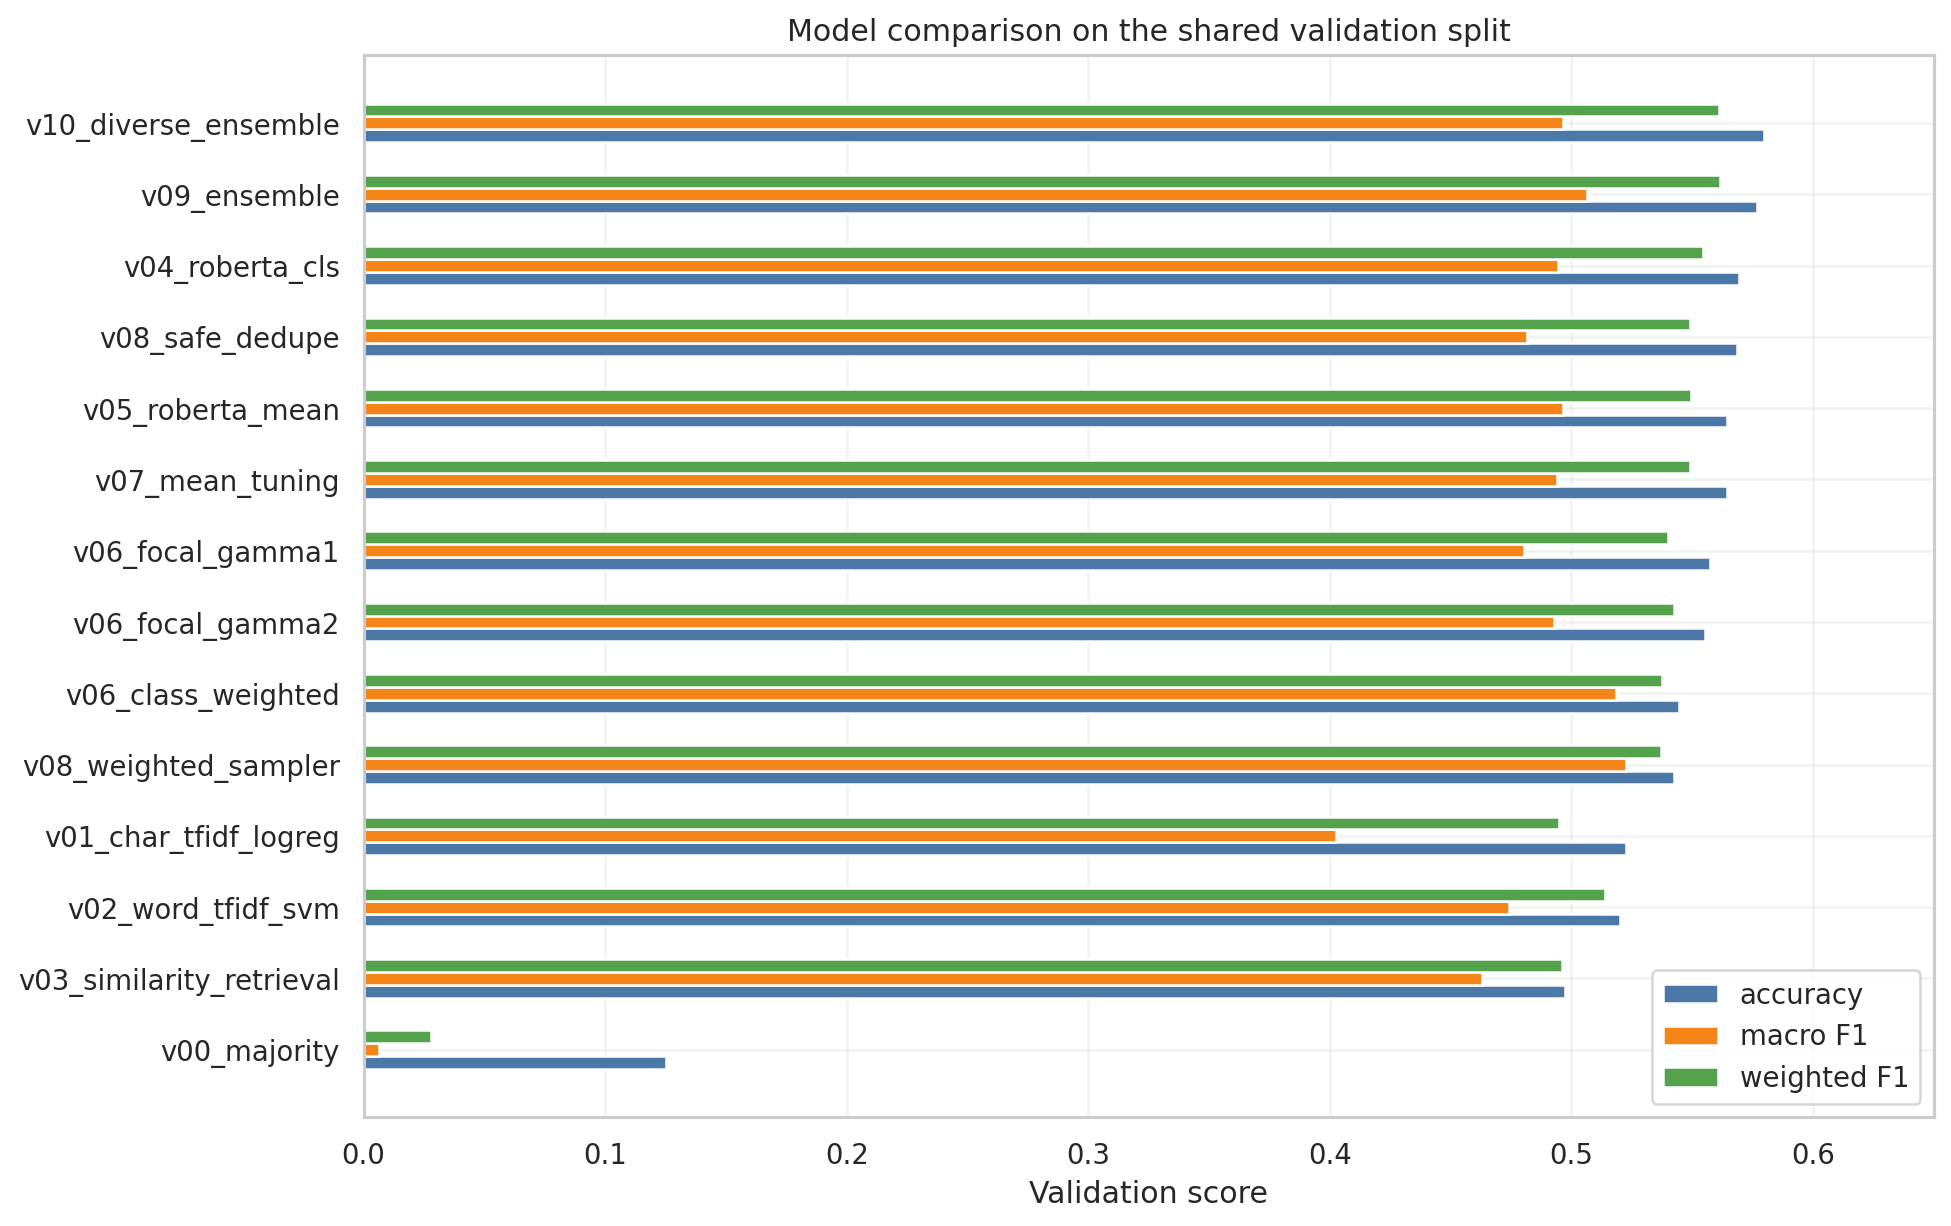
\includegraphics[width=\columnwidth]{figures/fig_10_model_comparison.png}
\caption{Validation comparison across model families.}
\label{fig:modelcomparison}
\end{figure}

The result was not simply ``deep learning beats everything''. Character and word TF--IDF remained competitive and became valuable ensemble members. The result was useful even when those models were not the final model because they showed that, in short clinical literals, surface form still matters.

The v10 search produced two important variants. The strongest validation-accuracy recipe was \texttt{vote\_diverse\_no\_retrieval\_val\_weighted}, with accuracy 0.583577, macro-F1 0.501074, and weighted-F1 0.564988. The final public candidate was \texttt{vote\_diverse\_no\_retrieval}, with validation accuracy 0.579562 and the best verified public score, 0.587. We report this distinction explicitly because internal validation and public leaderboard evidence are related but not identical.

\section{Error Analysis and Interpretability}

The evaluation notebook asks: \emph{Which model should we trust as our final submission?} To answer it, we inspected confusion matrices, per-class recall, confidence distributions, and real examples. Figure~\ref{fig:confusion} shows the final confusion matrix. Figure~\ref{fig:recall} shows that performance is uneven across categories, which is expected from the long tail.

\begin{figure}[h]
\centering
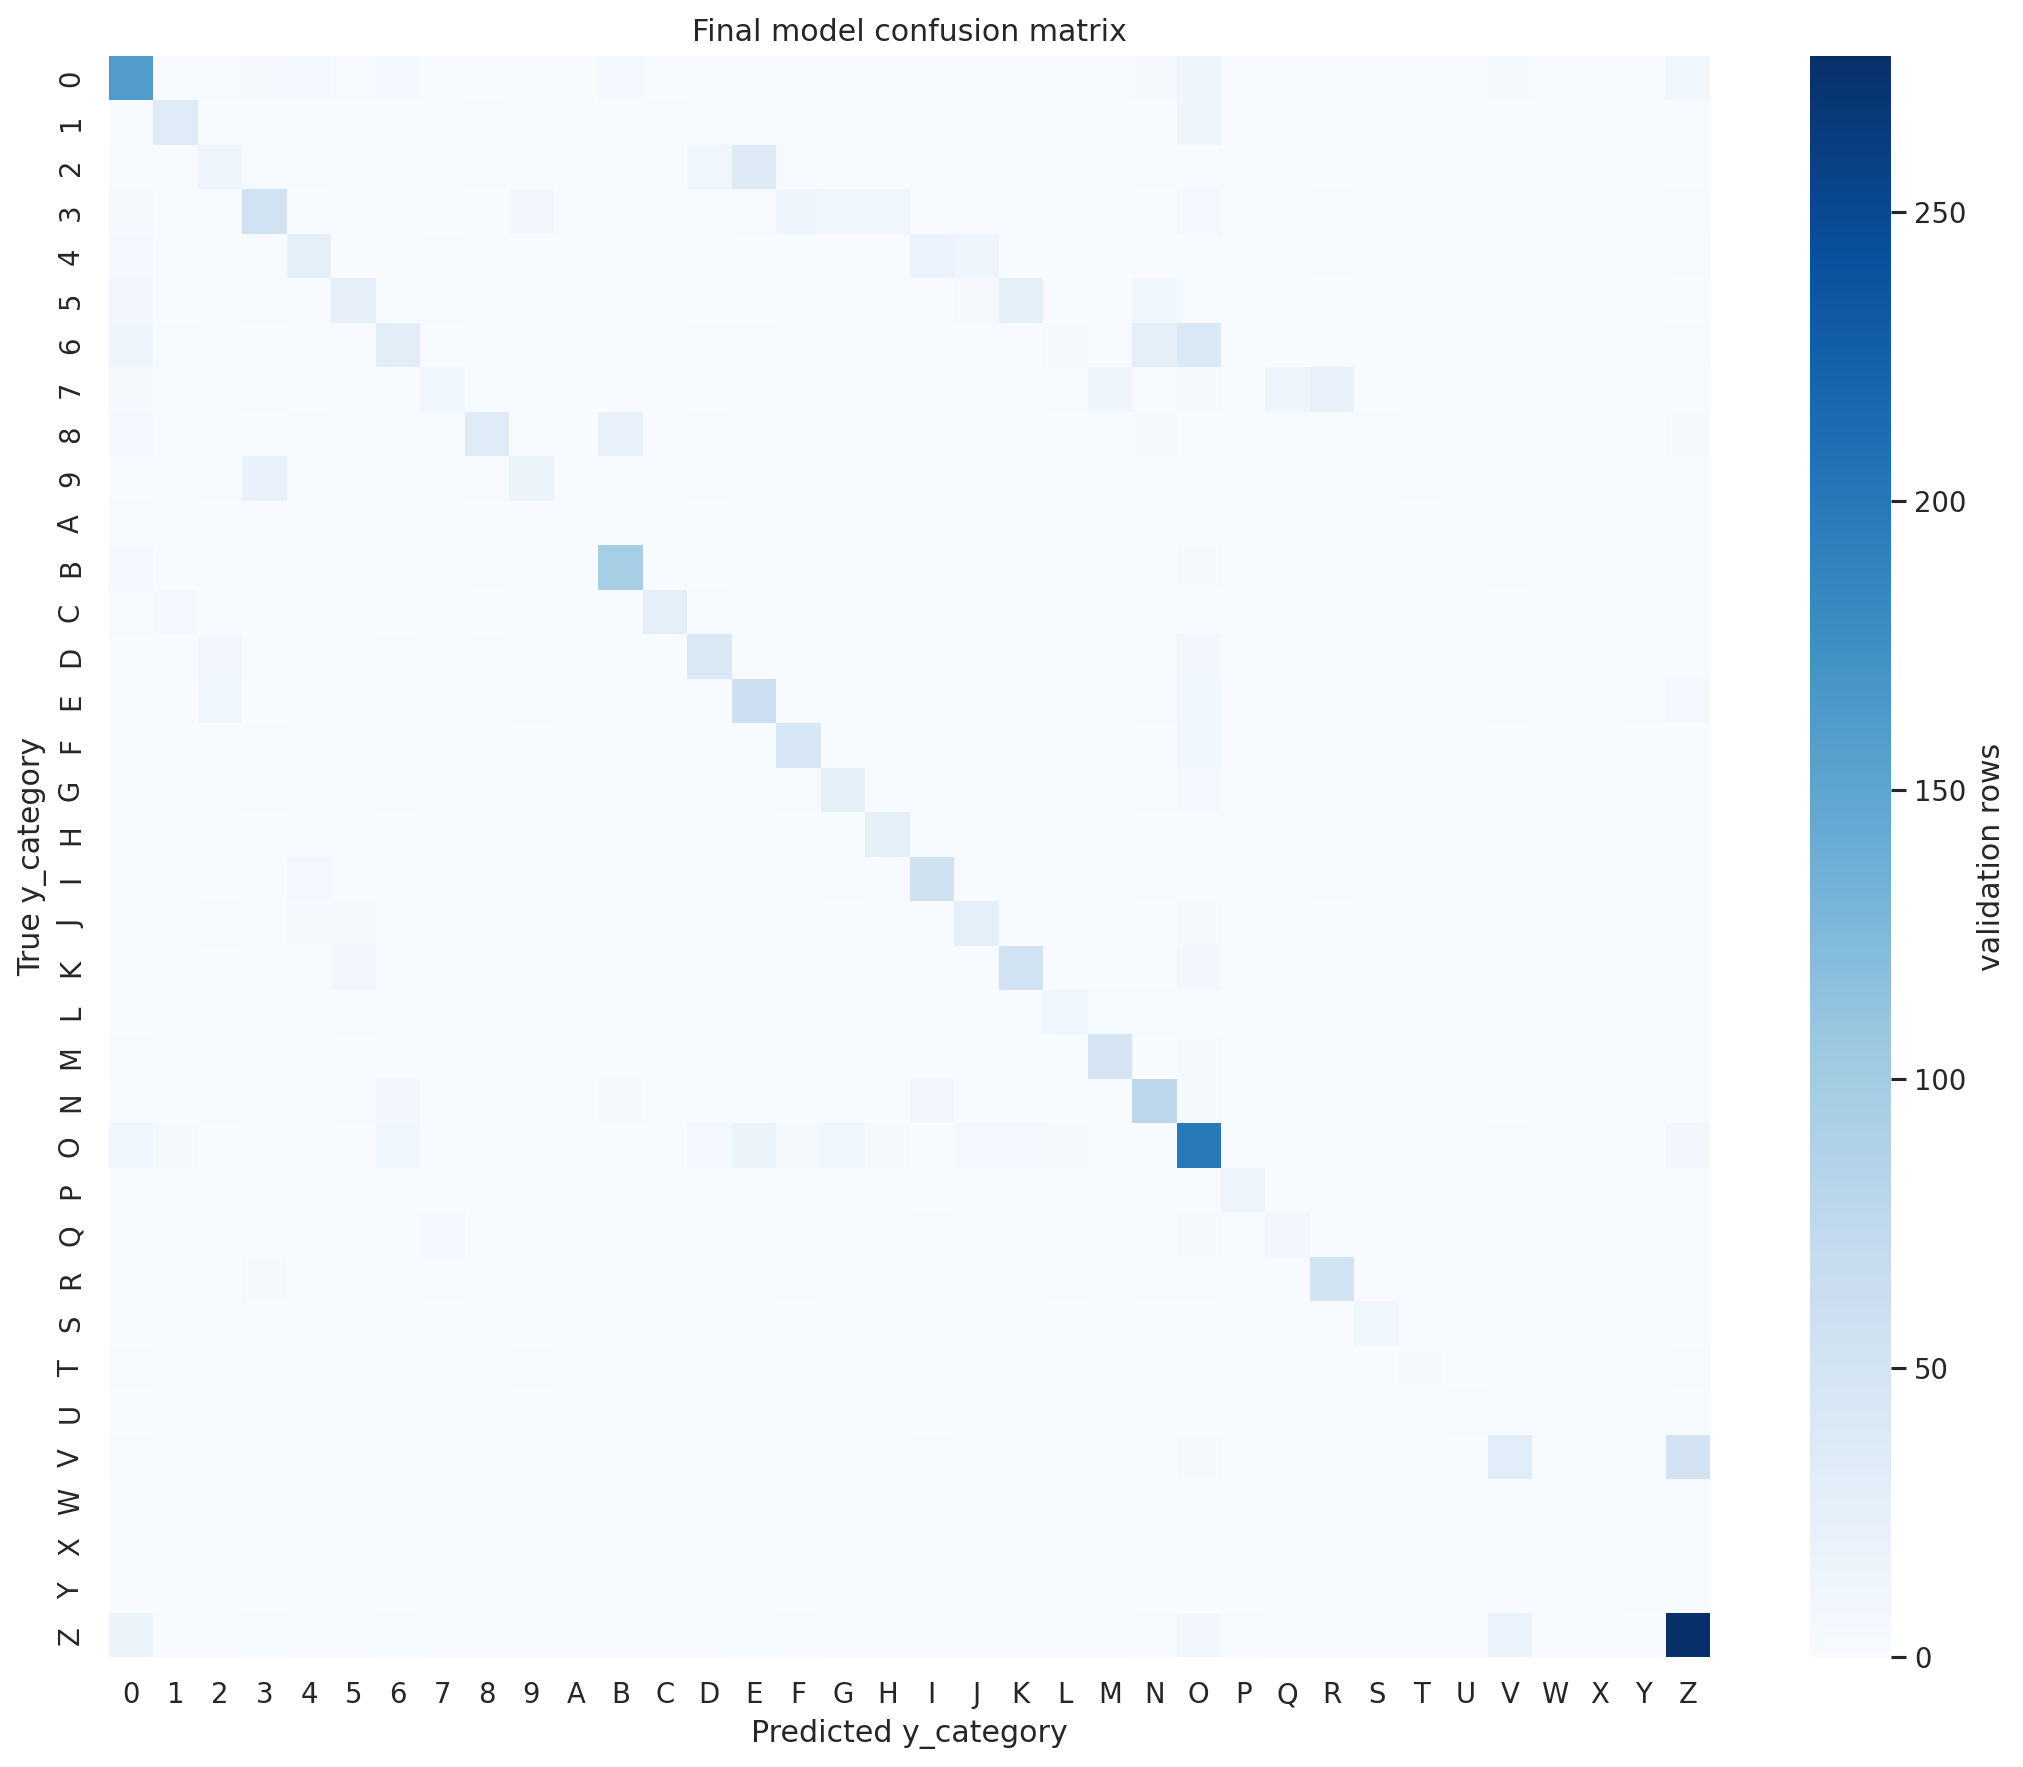
\includegraphics[width=\columnwidth]{figures/fig_11_final_confusion_matrix.png}
\caption{Confusion matrix for the final candidate. Confusions reflect broad ICD-prefix overlap and rare labels.}
\label{fig:confusion}
\end{figure}

\begin{figure}[h]
\centering
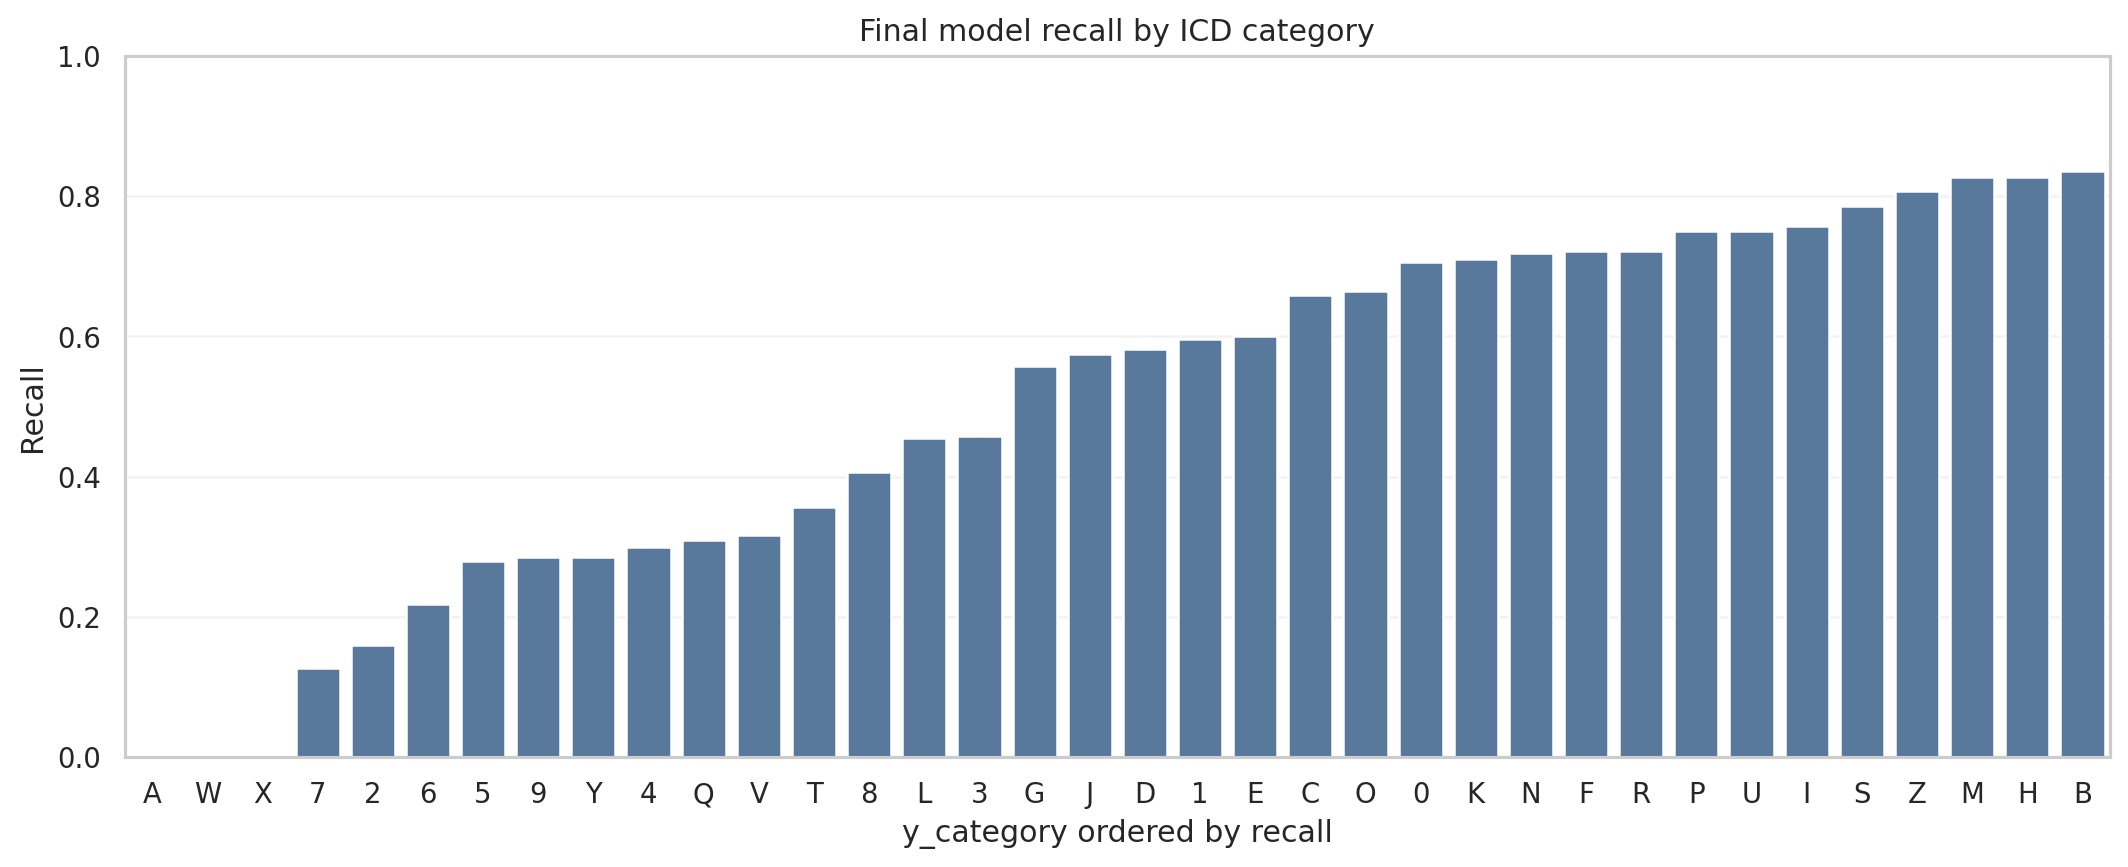
\includegraphics[width=\columnwidth]{figures/fig_12_per_class_recall.png}
\caption{Per-class recall for the final candidate. Macro-F1 is important because frequent classes can hide weak rare-class behavior.}
\label{fig:recall}
\end{figure}

Confidence analysis in Figure~\ref{fig:confidence} showed that high confidence does not guarantee correctness. Some wrong high-confidence examples are especially important in a hospital setting because they may look reliable to users. The typical causes of error were ambiguous literals, insufficient context, abbreviations, class imbalance, similar categories, and broad ICD-prefix granularity.

\begin{figure}[h]
\centering
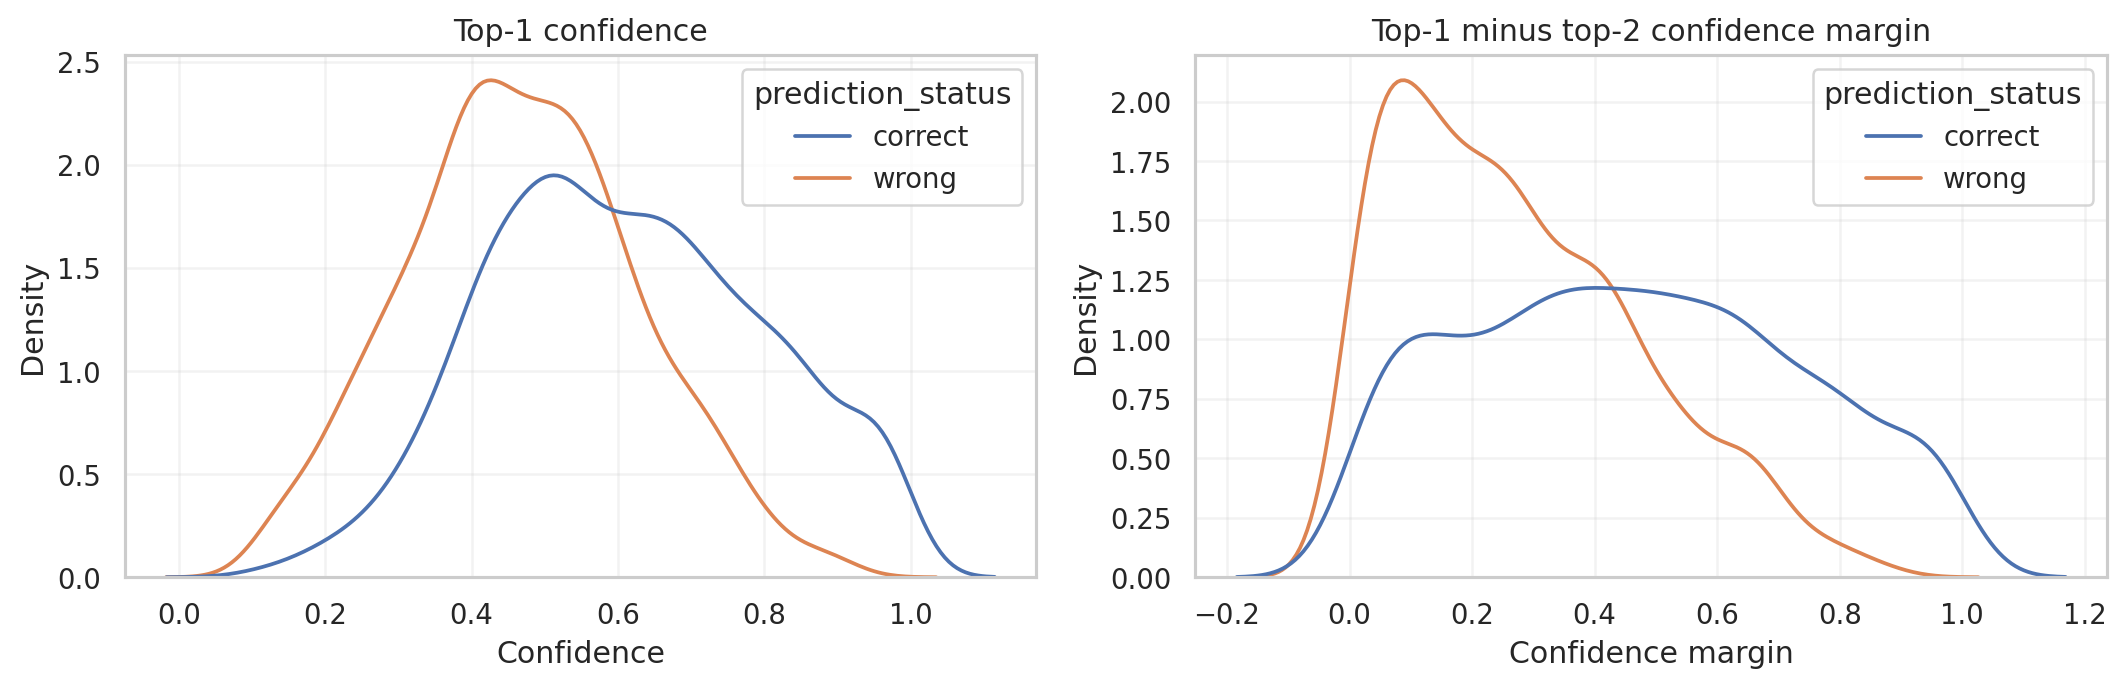
\includegraphics[width=\columnwidth]{figures/fig_13_confidence_correct_vs_wrong.png}
\caption{Confidence distributions for correct and incorrect predictions. Confidence is useful diagnostically, but not a clinical explanation.}
\label{fig:confidence}
\end{figure}

We treat interpretability carefully. Confusion matrices, margins, nearest examples, and feature weights are useful diagnostics, but they are not proof of medical reasoning. If attention or token attribution is added later, it should be presented with limitations rather than as a faithful explanation of clinical causality.

The most frequent confusion pairs also made clinical sense at the surface level. Table~\ref{tab:confusions} shows examples: \texttt{V} was often confused with \texttt{Z} for literals such as \emph{prótesis mamarias} and \emph{alergia Àcars}; \texttt{6} was confused with \texttt{O} for pregnancy-related literals such as \emph{patología fetal parto}; and \texttt{2} was confused with \texttt{E} for endocrine/metabolic-looking literals such as \emph{DIABETES}. Figure~\ref{fig:topconfusions} visualizes the top confused pairs.

\begin{table}[h]
\centering
\caption{Top observed confusion pairs for the final candidate.}
\label{tab:confusions}
\begin{tabularx}{\columnwidth}{ccrX}
\toprule
True & Pred. & Count & Example literals \\
\midrule
V & Z & 51 & prótesis mamarias; alergia Àcars \\
6 & O & 40 & patología fetal parto; preclampsia \\
2 & E & 35 & DIABETES; déficit de ácido fólico \\
6 & N & 26 & endometriosis; prolapso uteri \\
5 & K & 24 & esteatosis hepática; hernia inguinal \\
\bottomrule
\end{tabularx}
\end{table}

\begin{figure}[h]
\centering
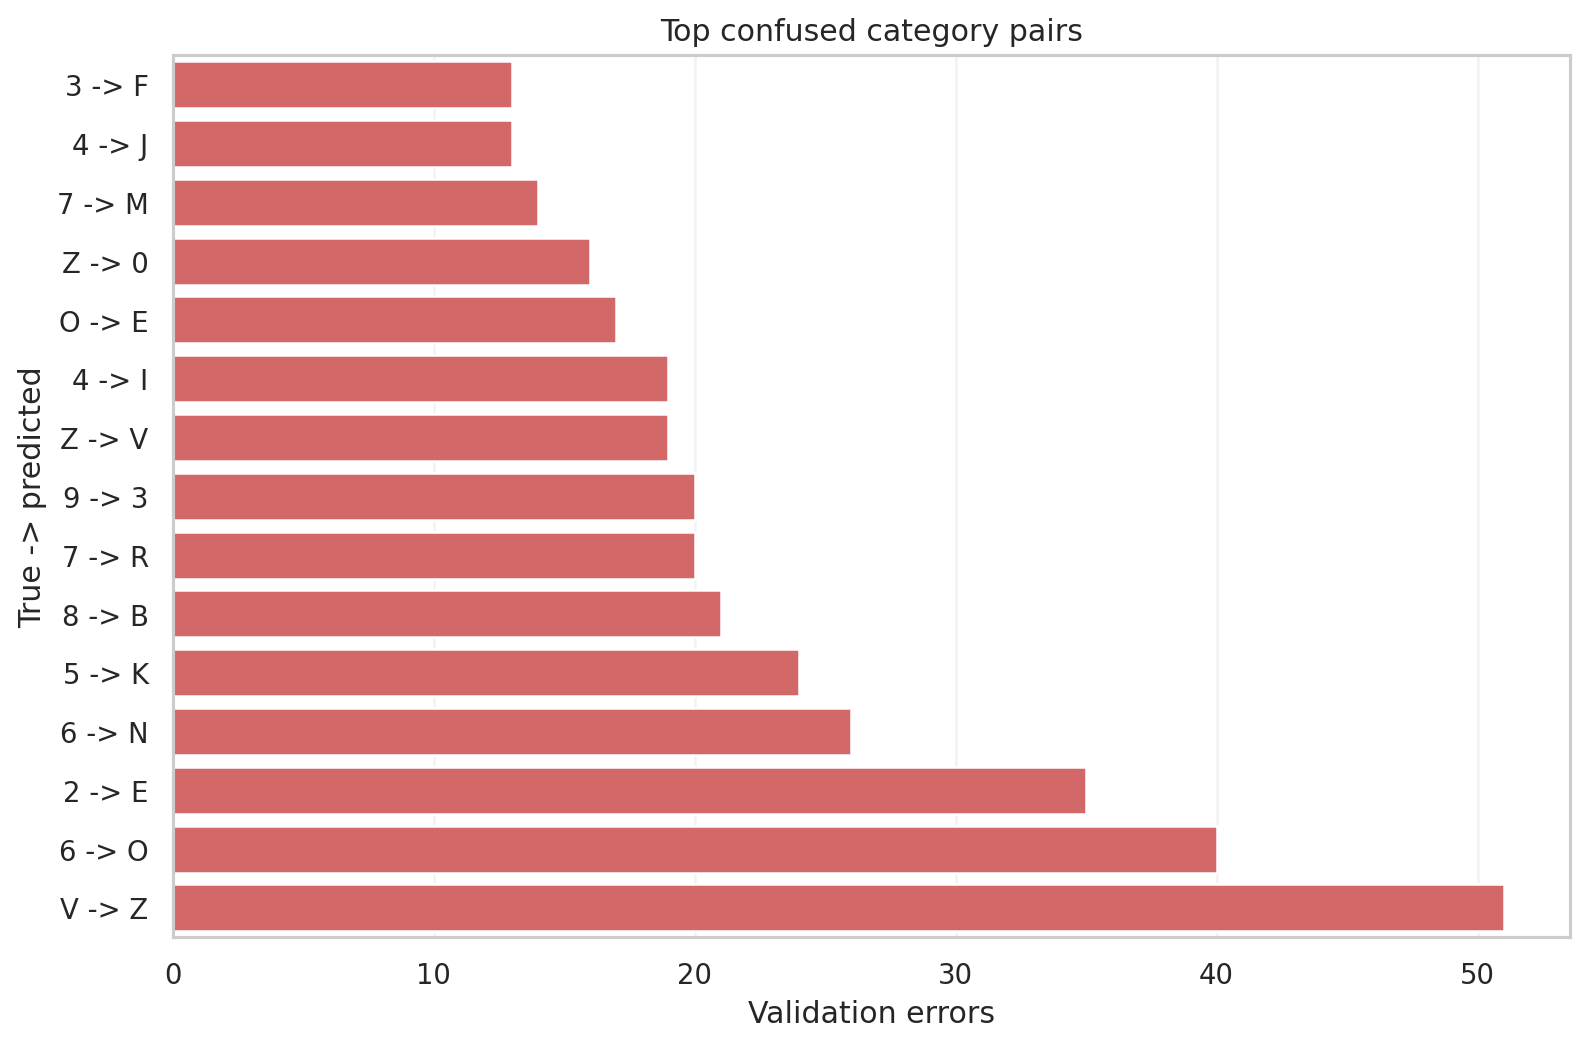
\includegraphics[width=\columnwidth]{figures/fig_15_top_confused_pairs.png}
\caption{Top confused category pairs. The plot was generated from validation predictions, not from leaderboard labels.}
\label{fig:topconfusions}
\end{figure}

\section{Final System and Kaggle Submission}

The final submission file is:
\begin{lstlisting}
submissions/final_submission.csv
\end{lstlisting}
The detailed leaderboard predictions are:
\begin{lstlisting}
outputs/predictions/final_leaderboard_detailed.csv
\end{lstlisting}

The final Kaggle submission file contains exactly:
\begin{lstlisting}
id, y_category
\end{lstlisting}
The best verified public score is 0.587 for \texttt{v10\_vote\_diverse\_no\_retrieval}. We do not state a final private ranking because no verified private leaderboard evidence is stored.

\section{What Would Happen in a Hospital?}

In a hospital, a system like this could help professional coders by suggesting candidate categories, highlighting uncertain cases, and making routine coding faster. It could improve consistency in records, accelerate statistics, and support DRG-related administrative workflows. That is the positive scenario, but it only makes sense if the system is designed as support.

The risks are equally real. A wrong code may affect reimbursement, hospital management indicators, quality statistics, or downstream clinical data reuse. If users trust the model too much, high-confidence errors could become harmful. Privacy is also central: clinical text must be handled under strict governance, with access control and anonymization where appropriate. Bias is another risk: if some categories, services, or language styles are underrepresented, the model may perform worse for them. For these reasons, the system should support professionals, not replace them. Interpretability tools should help review decisions, but human accountability remains necessary.

\section{Limitations}

First, the target is only the broad ICD prefix, not the full ICD code. This makes the competition tractable but less clinically specific than real coding. Second, the inputs are short literals, so many examples lack the context needed for confident coding. Third, we did not implement a full ICD hierarchy model, GNN, knowledge graph, or label-description matching system, although the ICD catalogue file makes some future work possible. Fourth, we did not compare with podium teams' models or ensemble with other teams' predictions because those models were not available in the repository. Fifth, public leaderboard feedback is not a substitute for a final private leaderboard result.

\section{Future Work}

Future work follows directly from these limitations. We could predict full ICD codes rather than only prefixes, use ICD descriptions more explicitly, model hierarchy through parent--child relations or graph neural networks, add calibrated confidence thresholds for human review, and compare with other teams' methods if allowed. Another promising path is a retrieval-augmented model that proposes similar historical literals and ICD descriptions together with the predicted category. Any augmentation should remain clinically safe: we would avoid random deletion, unverified synonym replacement, or changes that affect negation.

\section{Conclusion and Reflection}

This project became more than a leaderboard exercise. We started with a basic baseline and a short presentation, received feedback that our direction was reasonable, and then built a complete NLP workflow around the data. The final result was a diverse ensemble with the best verified public score in our repository, but the deeper value was understanding why each step mattered.

We are grateful for the practical activity because it grounded course concepts in a real application. Text processing was not just regex; it was the decision not to destroy accents, punctuation, and abbreviations. Transformers were not just architecture diagrams; they were a way of reusing biomedical Spanish language knowledge. Evaluation was not just a number; it was a way of seeing which clinical categories and examples remained fragile.

Language is part of human life, and in healthcare it becomes part of memory, organization, payment, and care. That makes NLP powerful, but also responsible. Our final system is not ready for clinical deployment, but it is a traceable academic prototype showing how classical NLP and pretrained biomedical language models can work together on ICD category codification.

\section*{Appendix: Reproducibility Commands}

\begin{lstlisting}[language=bash]
python -m venv .venv
source .venv/bin/activate
pip install -r requirements.txt

python scripts/analyze_data_annotations.py
python scripts/run_preprocessing.py
python scripts/analyze_tokenization.py

python models/v00_majority_baseline.py
python models/v01_tfidf_char_logreg.py
python models/v02_tfidf_word_svm.py
python models/v03_similarity_retrieval_baseline.py

python models/v04_roberta_cls.py
python models/v05_roberta_mean.py
python models/v06_roberta_mean_imbalance_aware.py
python models/v07_roberta_mean_tuning.py
python models/v08_roberta_mean_augmented.py
python models/v09_ensemble.py
python models/v10_diverse_ensemble_search.py

python -m src.evaluation

kaggle competitions submit \
  -c uab-asho-ai-codification \
  -f submissions/final_submission.csv \
  -m "Team 10 final public-best v10 diverse ensemble"
\end{lstlisting}

\bibliographystyle{plain}
\bibliography{references}

\end{document}
